\section{Failed optimizations}
Two memory optimizations were attempted without achieving any performance gains.
They still provided useful information on how

\subsection{Contiguous acces using warp level primitives} \label{sec:contuguous_access}
As we want to operate on 32-bit values and each pixel is stored as a 10-bit value, each thread is processing 160 bits, or five words, as it is the lowest common multiple of 32 and 10.
Thus every thread reads five consecutive words as shown:
\begin{align}
    a_T[i] = d[T*5+i], &  & i \in (0,1,2,3,4)
\end{align}
Where $T$ is the thread index in the warp, $a_T$ is the local memory of thread $T$, and $d$ is the relevant segment of the image stored in device memory.

It was hypothesized that it would be faster to let first read the data contiguously into shared memory and then redistribute it as follows:
\begin{align}
    s[i*32+T] & = d[i*32+T],  & i & \in (0,1,2,3,4) \\
    a_T[i]    & = s[(T*5+i)], & i & \in (0,1,2,3,4)
    \label{eq:contiguous_reading}
\end{align}
Where $s$ is shared local memory.
However, this was not the case as the performance was actually worse than the non-contiguous reading.


A second attempt was done using the \code{__shfl_sync} function, which is a warp-level primitive used to exchange data between threads in a warp \cite{linUsingCUDAWarpLevel2018}.
As the data exchange is performed directly between registers, this is faster than going through shared memory \cite{linUsingCUDAWarpLevel2018}
Data was read contiguously into local buffers of each thread, then exchanged so every thread ended up with five consecutive words.
However, finding the right indices is hard as you need to specify what data to send and what thread to read from, rather than what data to read from what thread.
The full index table, shown in Table \ref{table:memory_index} in Appendix \ref{chap:additional_resources}, was created and studied in order to end up with the following formulation:
\begin{align}
    c_T[i] & = d[i*32+T],       &   &                   & i & \in (0,1,2,3,4) \\
    c_T[j] & \rightarrow a_x[i] & j & = (2 * (T -i))\%5 & i & \in (0,1,2,3,4) \\
    a_T[i] & \leftarrow c_j[x]  & j & = (T*5 + i)\%32   & i & \in (0,1,2,3,4)
    \label{eq:contiguous_reading_shfl}
\end{align}
where $x$ represents the thread the data is sent to.
The code equivalent to this is written as follows.
\begin{minted}[linenos=false]{cuda}
    a[i] = __shfl_sync(0xffffffff, c[2(*(T-i))%5], (T*5 + i)%32);
\end{minted}



The reason why coalesced memory access using the \code{__shfl_sync} operation is slower than non-coalesced memory access is believed to be due to the effectiveness of caching in mitigating the cost of non-coalesced access. This hypothesis finds support in Volkov's thesis, specifically in the section titled "Unstructured memory access," where it demonstrates that the cost of unstructured memory access is significantly reduced for smaller data transactions \cite[Sec 6.7]{volkovLatencyHiding2016}.

To verify this hypothesis, I intended to utilize the \gls{nsight} tool to create a memory chart, like the one in Figure \ref{fig:cache_hits}. However, it was not feasible as this feature is only available for NVIDIA \glspl{gpu} with compute capability 7.5 or greater while the \jx has to compute capability 7.2 \cite{crovellaUsingNsightCompute2019}\cite{CUDA2023}.


\begin{figure}[H]
    \centering
    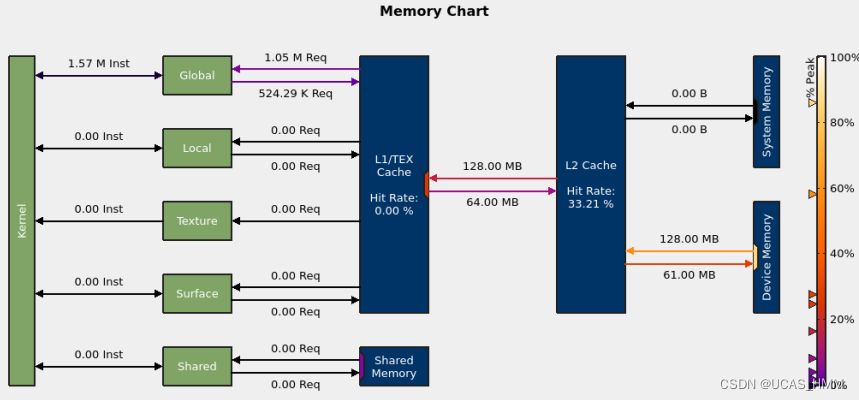
\includegraphics[width=\textwidth]{figures/cuda/cache_hits.png}
    \caption{Illustrative example of memorychart generated with \gls{nsight}. \cite{nv-computeNsightComputeMemory2022}}
    \label{fig:cache_hits}
\end{figure}


\subsection{Use of constant memory}
During the development process, it was tested whether storing the constant values used in the debayer algorithm in constant memory would speed up the process.
Constant memory is a type of limited read-only memory available on NVIDIA \glsps{gpu} \cite[61]{nvidiaCUDABestPractices2023}.
NVIDIA \glspl{gpu} only have 64KiB of constant memory \cite[61]{nvidiaCUDABestPractices2023}.
Read instructions from constant memory are very efficient, and the best performance is achieved when all threads in a warp, as opposed to regular memory where this would result in inefficient collisions \cite[61]{nvidiaCUDABestPractices2023} \cite[13,14]{volkovLatencyHiding2016}.
This would be the case for the debayer algorithm as all threads in a warp read the same constant values.

All unique constant variables used in the algorithm were collected as a part of the automatic code generation and stored in a constant device array.
Unfortunately, this change had no visible impact on the performance.
A minimal test was later created that performed a very simple repeated multiply and added operation, where the coefficient and constants were either stored in constant memory or defined as literal variables in the function as shown in \code{mfa_1} and \code{mfa_2} in Listing \ref{listing:cuda_mem_tests}.
These minimal tests showed that using constant memory was actually marginally slower (0.08\% on average) than using literal values.

Further, it was tested whether storing the coefficient in constant variables would improve performance as there is no built-in \code{__half2} literal type, as shown in \code{mfa_3} in Listing \ref{listing:cuda_mem_tests}.
This gave marginally better results than \code{mfa_1} (0.04\% on average) but was ignored as it was not worth the effort to implement in the code generator.

\begin{listing}[H]
    \begin{minted}{cuda}
        __device__ __forceinline__ __half2 mfa_1(__half2 a) {
        return __hfma2(__float2half2_rn(0.098f), a, __float2half2_rn(3.14f));
        }
        __device__ __forceinline__ __half2 mfa_2(__half2 a) {
            return __hfma2(constant_mem[0], a, constant_mem[1]);
        }
        __device__ __forceinline__ __half2 mfa_3(__half2 a) {
            const __half2 b = __float2half2_rn(0.098f);
            const __half2 c = __float2half2_rn(3.14f);
            return __hfma2(b, a, c);
        }
    \end{minted}
    \caption{Small functions used to test different memory implementations.}
    \label{listing:cuda_mem_tests}
\end{listing}




